% Captions for the five D1-bis result figures (fig5-fig9).
% Paste each block into the relevant section of the manuscript.
% Numbers come exclusively from frozen artifacts: results/m4_report.json
% (commit f6145a5), results/a1_*.json (commit e418579), docs/15
% sections 1.1 and 3, docs/16 (inter-run rule).

% ---------------------------------------------------------------- fig 5 ---
\begin{figure}[t]
\centering
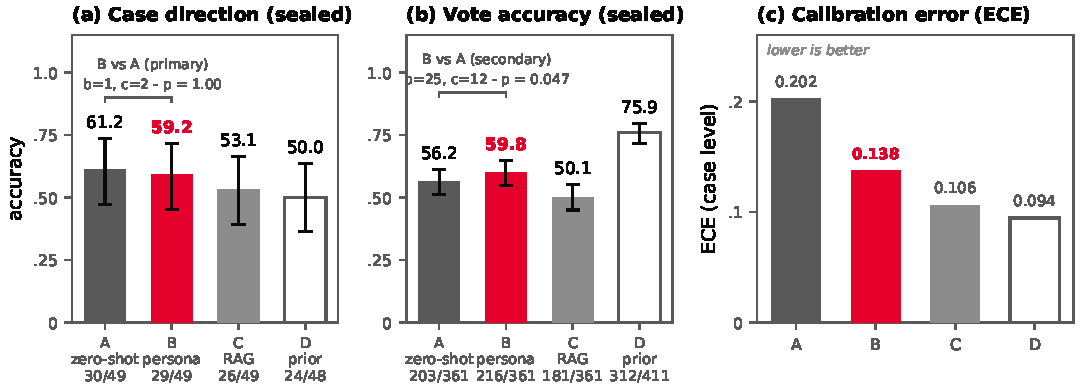
\includegraphics[width=\linewidth]{figures/fig5_m4_primary.pdf}
\caption{\textbf{Primary result on the sealed 5--4 exam (phase S,
$n=50$).} Accuracy of the four pre-registered conditions with Wilson
95\% intervals: A~(zero-shot), B~(persona: biographical prompt + QLoRA
adapter), C~(RAG), D~(per-justice ideological prior, drawn hollow as a
reference rule rather than a language model). \emph{(a)}~Case-direction
accuracy, the primary endpoint: the pre-registered McNemar test of B
vs.\ A is null ($b=1$, $c=2$, $p=1.00$) --- personalization does not
significantly improve case-level prediction on close cases. \emph{(b)}
Vote-level accuracy (D evaluated on $n=411$ votes including historical
justices; A/B/C on $n=361$): the secondary, vote-level McNemar test is
nominally significant ($b=25$, $c=12$, $p=.047$) and the trivial
per-justice prior D dominates every language condition.
\emph{(c)}~Expected calibration error at the case level (lower is
better; vote-level ECE: A~.226, B~.169, C~.137, D~.094). All conditions
are poorly calibrated; the prior rule is the best calibrated of the
four.}
\label{fig:m4-primary}
\end{figure}

% ---------------------------------------------------------------- fig 6 ---
\begin{figure}[t]
\centering
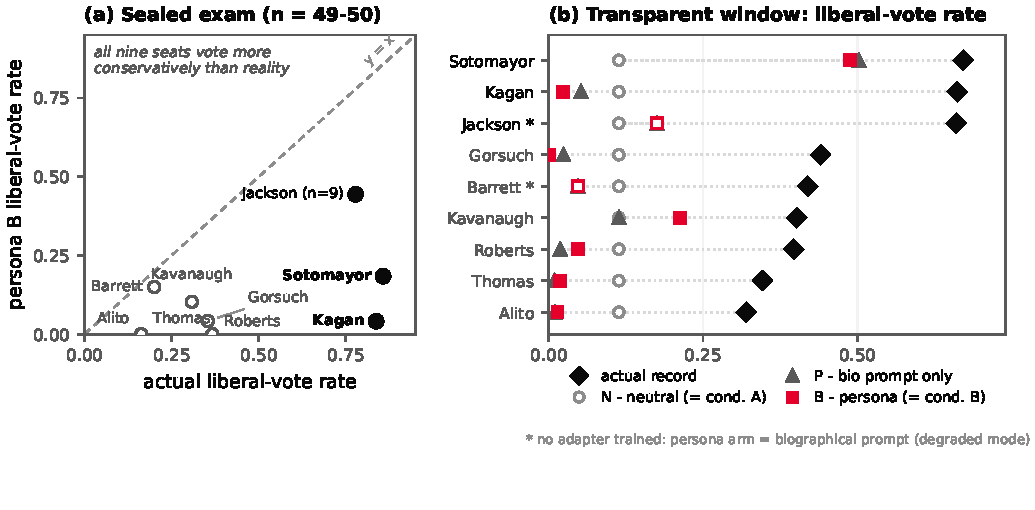
\includegraphics[width=\linewidth]{figures/fig6_ideological_dial.pdf}
\caption{\textbf{The ideological dial: actual vs.\ simulated
liberal-vote rates.} \emph{(a)}~On the sealed exam, every seat's
persona (condition B) votes more conservatively than the justice it
imitates; filled markers denote the liberal bloc. The persona-predicted
rate never exceeds 0.44 while the actual rate spans 0.16--0.86
(Jackson: $n=9$ votes). \emph{(b)}~The same dial, decomposed on the
transparent window ($n=211$ casefiles, sealed cases excluded): the
actual record, the neutral arm N ($\equiv$ condition A scheme), the
biographical prompt alone (P), and the full persona B (E1 arm
``A'', byte-identical to condition B). The base model pins every seat
near $0.11$; the prompt moves Sotomayor to $0.50$ but barely moves
Kagan ($0.05$); the adapter's marginal pull on top of the prompt is
small everywhere (Gorsuch ends at $0.00$). Actual rates are derived from
the frozen corpus and validated exactly against the published E1
arm-N accuracies. \emph{Barrett and Jackson have no adapter (degraded,
pre-inscribed mode): their persona arm \emph{is} the biographical
prompt} (open red squares).}
\label{fig:dial}
\end{figure}

% ---------------------------------------------------------------- fig 7 ---
\begin{figure}[t]
\centering
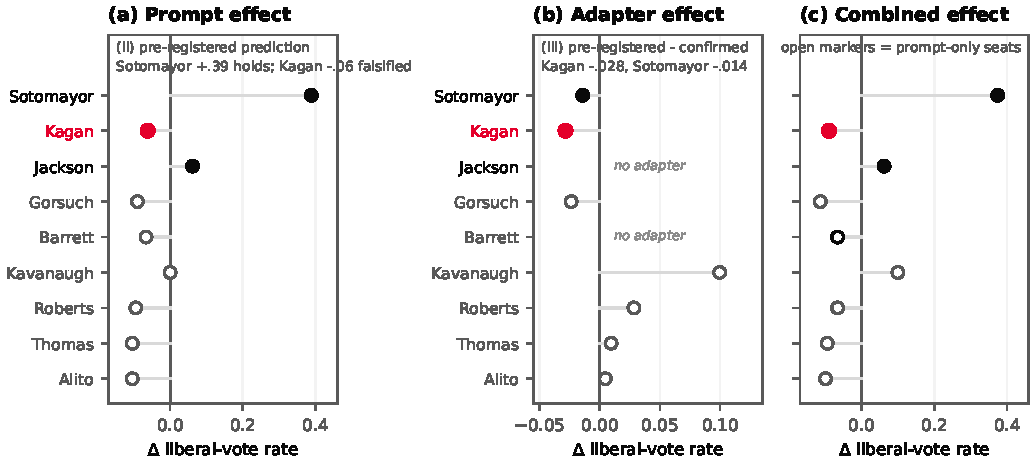
\includegraphics[width=\linewidth]{figures/fig7_prompt_vs_adapter.pdf}
\caption{\textbf{E1: causal decomposition of the dial (transparent
window, $n=211$; single run, seed 271828).} Change in predicted
liberal-vote rate per seat. \emph{(a)}~Prompt effect $\Delta(P-N)$: the
pre-registered prediction (ii) --- the biography lifts liberal seats
--- holds spectacularly for Sotomayor ($+0.39$) and modestly for
Jackson ($+0.06$), but is \emph{falsified for Kagan} ($-0.06$),
highlighted in red. \emph{(b)}~Adapter effect $\Delta(B-P)$: the
marginal effect of adding the adapter on top of the prompt is small
everywhere ($\le +0.10$) and negative for the two pre-registered
targets, confirming prediction (iii) --- the adapter erases the
prompt's gain for Kagan ($-0.028$) and Sotomayor ($-0.014$).
\emph{(c)}~Combined effect $\Delta(B-N)$; open markers mark the
prompt-only seats (Barrett, Jackson --- no adapter exists). Arms:
N~$=$ neutral base model ($\equiv$ condition A scheme; conservative
default $0.114$ for all seats --- prediction (i), confirmed), P~$=$
biographical prompt, B~$=$ persona (E1 artifact arm ``A'' $\equiv$
condition B). Identity injected in the prompt is not behavior learned
by the adapter.}
\label{fig:decomposition}
\end{figure}

% ---------------------------------------------------------------- fig 8 ---
\begin{figure}[t]
\centering
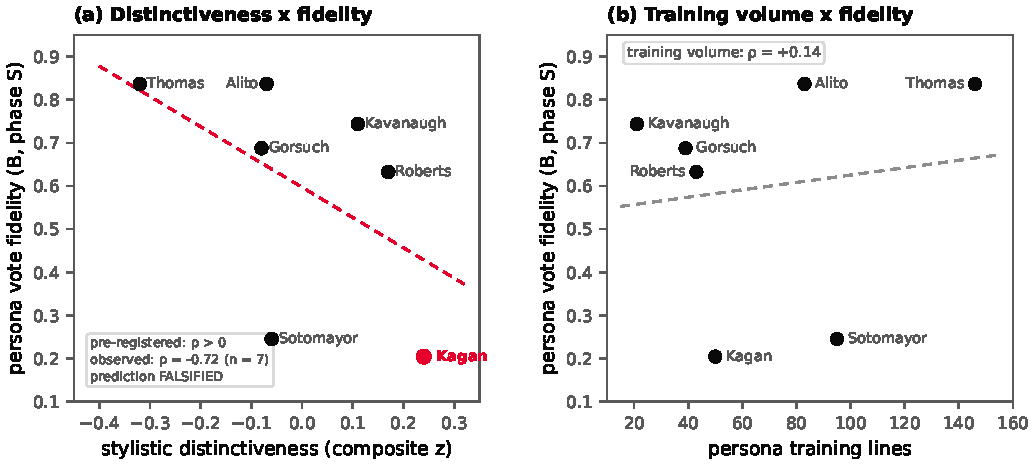
\includegraphics[width=\linewidth]{figures/fig8_e2_distinctiveness.pdf}
\caption{\textbf{E2: stylistic distinctiveness does not predict persona
fidelity --- a pre-registered prediction, falsified ($n=7$
adapters).} \emph{(a)}~Composite stylistic distinctiveness (lexical
richness, sentence-length variance, function-word and
authorial-marker signatures, TF-IDF/JSD distance to the other judges)
against persona vote fidelity on the sealed exam. The pre-registered
prediction was a \emph{positive} correlation; the observed Spearman
correlation is $\rho=-0.72$ in phase S ($-0.61$ in phase T). Kagan is
the most distinctive writer and the worst persona; Thomas the least
distinctive and among the best. \emph{(b)}~Training volume explains
nothing ($\rho=+0.14$). The surface style transfers; the decision
function does not: persona fidelity tracks the justice's alignment
with the base model's conservative default, not the distinctiveness of
the pen. Exploratory label (measures chosen after observing
fidelities; the correlation predictions themselves were committed to
the repository before execution).}
\label{fig:e2}
\end{figure}

% ---------------------------------------------------------------- fig 9 ---
\begin{figure}[t]
\centering
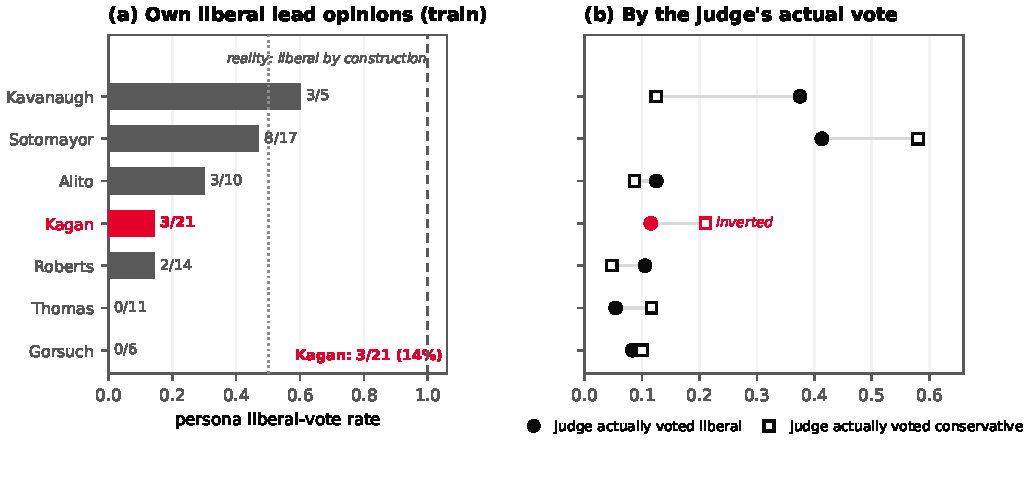
\includegraphics[width=\linewidth]{figures/fig9_e3_autocoherence.pdf}
\caption{\textbf{E3: auto-coherence probe --- the persona does not
reproduce the judge's votes even on the cases it was trained on
(pre-specified, exploratory).} \emph{(a)}~Persona liberal-vote rate on
the training cases where the justice authored the lead opinion
\emph{and} voted liberal; by construction the actual rate is 1.0
(dashed line). Kagan's persona, trained on 21 such opinions, votes
liberal on 3 of 21 (14\%). No persona reaches even two-thirds.
\emph{(b)}~The persona's liberal-vote rate split by the judge's actual
vote on his or her own training cases: for Kagan the relationship is
\emph{inverted} --- her persona votes liberal more often on cases where
she voted conservative (21\%) than on cases where she voted liberal
(12\%). The same inversion affects Sotomayor, Thomas and Gorsuch
(4 of 7 adapters). The adapter has seen the judge's words on these
very cases; it did not learn the vote that produced them.}
\label{fig:e3}
\end{figure}
